\documentclass[twoside]{book}

% Packages required by doxygen
\usepackage{fixltx2e}
\usepackage{calc}
\usepackage{doxygen}
\usepackage[export]{adjustbox} % also loads graphicx
\usepackage{graphicx}
\usepackage[utf8]{inputenc}
\usepackage{makeidx}
\usepackage{multicol}
\usepackage{multirow}
\PassOptionsToPackage{warn}{textcomp}
\usepackage{textcomp}
\usepackage[nointegrals]{wasysym}
\usepackage[table]{xcolor}

% Font selection
\usepackage[T1]{fontenc}
\usepackage[scaled=.90]{helvet}
\usepackage{courier}
\usepackage{amssymb}
\usepackage{sectsty}
\renewcommand{\familydefault}{\sfdefault}
\allsectionsfont{%
  \fontseries{bc}\selectfont%
  \color{darkgray}%
}
\renewcommand{\DoxyLabelFont}{%
  \fontseries{bc}\selectfont%
  \color{darkgray}%
}
\newcommand{\+}{\discretionary{\mbox{\scriptsize$\hookleftarrow$}}{}{}}

% Page & text layout
\usepackage{geometry}
\geometry{%
  a4paper,%
  top=2.5cm,%
  bottom=2.5cm,%
  left=2.5cm,%
  right=2.5cm%
}
\tolerance=750
\hfuzz=15pt
\hbadness=750
\setlength{\emergencystretch}{15pt}
\setlength{\parindent}{0cm}
\setlength{\parskip}{3ex plus 2ex minus 2ex}
\makeatletter
\renewcommand{\paragraph}{%
  \@startsection{paragraph}{4}{0ex}{-1.0ex}{1.0ex}{%
    \normalfont\normalsize\bfseries\SS@parafont%
  }%
}
\renewcommand{\subparagraph}{%
  \@startsection{subparagraph}{5}{0ex}{-1.0ex}{1.0ex}{%
    \normalfont\normalsize\bfseries\SS@subparafont%
  }%
}
\makeatother

% Headers & footers
\usepackage{fancyhdr}
\pagestyle{fancyplain}
\fancyhead[LE]{\fancyplain{}{\bfseries\thepage}}
\fancyhead[CE]{\fancyplain{}{}}
\fancyhead[RE]{\fancyplain{}{\bfseries\leftmark}}
\fancyhead[LO]{\fancyplain{}{\bfseries\rightmark}}
\fancyhead[CO]{\fancyplain{}{}}
\fancyhead[RO]{\fancyplain{}{\bfseries\thepage}}
\fancyfoot[LE]{\fancyplain{}{}}
\fancyfoot[CE]{\fancyplain{}{}}
\fancyfoot[RE]{\fancyplain{}{\bfseries\scriptsize Generated by Doxygen }}
\fancyfoot[LO]{\fancyplain{}{\bfseries\scriptsize Generated by Doxygen }}
\fancyfoot[CO]{\fancyplain{}{}}
\fancyfoot[RO]{\fancyplain{}{}}
\renewcommand{\footrulewidth}{0.4pt}
\renewcommand{\chaptermark}[1]{%
  \markboth{#1}{}%
}
\renewcommand{\sectionmark}[1]{%
  \markright{\thesection\ #1}%
}

% Indices & bibliography
\usepackage{natbib}
\usepackage[titles]{tocloft}
\setcounter{tocdepth}{3}
\setcounter{secnumdepth}{5}
\makeindex

% Hyperlinks (required, but should be loaded last)
\usepackage{ifpdf}
\ifpdf
  \usepackage[pdftex,pagebackref=true]{hyperref}
\else
  \usepackage[ps2pdf,pagebackref=true]{hyperref}
\fi
\hypersetup{%
  colorlinks=true,%
  linkcolor=blue,%
  citecolor=blue,%
  unicode%
}

% Custom commands
\newcommand{\clearemptydoublepage}{%
  \newpage{\pagestyle{empty}\cleardoublepage}%
}

\usepackage{caption}
\captionsetup{labelsep=space,justification=centering,font={bf},singlelinecheck=off,skip=4pt,position=top}

%===== C O N T E N T S =====

\begin{document}

% Titlepage & ToC
\hypersetup{pageanchor=false,
             bookmarksnumbered=true,
             pdfencoding=unicode
            }
\pagenumbering{roman}
\begin{titlepage}
\vspace*{7cm}
\begin{center}%
{\Large My Project }\\
\vspace*{1cm}
{\large Generated by Doxygen 1.8.11}\\
\end{center}
\end{titlepage}
\clearemptydoublepage
\tableofcontents
\clearemptydoublepage
\pagenumbering{arabic}
\hypersetup{pageanchor=true}

%--- Begin generated contents ---
\chapter{Hierarchical Index}
\section{Class Hierarchy}
This inheritance list is sorted roughly, but not completely, alphabetically\+:\begin{DoxyCompactList}
\item \contentsline{section}{qa\+\_\+squitter\+\_\+select}{\pageref{classqa__squitter__select}}{}
\item squitter\+\_\+mux\begin{DoxyCompactList}
\item \contentsline{section}{gr\+:\+:squitter\+\_\+select\+:\+:squitter\+\_\+mux\+\_\+impl}{\pageref{classgr_1_1squitter__select_1_1squitter__mux__impl}}{}
\end{DoxyCompactList}
\end{DoxyCompactList}

\chapter{Class Index}
\section{Class List}
Here are the classes, structs, unions and interfaces with brief descriptions\+:\begin{DoxyCompactList}
\item\contentsline{section}{\hyperlink{classqa__squitter__select}{qa\+\_\+squitter\+\_\+select} \\*Collect all the tests for the gr-\/filter directory }{\pageref{classqa__squitter__select}}{}
\item\contentsline{section}{\hyperlink{classgr_1_1squitter__select_1_1squitter__mux__impl}{gr\+::squitter\+\_\+select\+::squitter\+\_\+mux\+\_\+impl} }{\pageref{classgr_1_1squitter__select_1_1squitter__mux__impl}}{}
\end{DoxyCompactList}

\chapter{File Index}
\section{File List}
Here is a list of all documented files with brief descriptions\+:\begin{DoxyCompactList}
\item\contentsline{section}{{\bfseries qa\+\_\+squitter\+\_\+select.\+h} }{\pageref{qa__squitter__select_8h}}{}
\item\contentsline{section}{\hyperlink{squitter__mux__impl_8cc}{squitter\+\_\+mux\+\_\+impl.\+cc} }{\pageref{squitter__mux__impl_8cc}}{}
\item\contentsline{section}{{\bfseries squitter\+\_\+mux\+\_\+impl.\+h} }{\pageref{squitter__mux__impl_8h}}{}
\end{DoxyCompactList}

\chapter{Class Documentation}
\hypertarget{classqa__squitter__select}{}\section{qa\+\_\+squitter\+\_\+select Class Reference}
\label{classqa__squitter__select}\index{qa\+\_\+squitter\+\_\+select@{qa\+\_\+squitter\+\_\+select}}


collect all the tests for the gr-\/filter directory  




{\ttfamily \#include $<$qa\+\_\+squitter\+\_\+select.\+h$>$}

\subsection*{Static Public Member Functions}
\begin{DoxyCompactItemize}
\item 
static Cpp\+Unit\+::\+Test\+Suite $\ast$ \hyperlink{classqa__squitter__select_a0f577a91ff587b225dea766670266871}{suite} ()\hypertarget{classqa__squitter__select_a0f577a91ff587b225dea766670266871}{}\label{classqa__squitter__select_a0f577a91ff587b225dea766670266871}

\begin{DoxyCompactList}\small\item\em return suite of tests for all of gr-\/filter directory \end{DoxyCompactList}\end{DoxyCompactItemize}


\subsection{Detailed Description}
collect all the tests for the gr-\/filter directory 

The documentation for this class was generated from the following files\+:\begin{DoxyCompactItemize}
\item 
qa\+\_\+squitter\+\_\+select.\+h\item 
qa\+\_\+squitter\+\_\+select.\+cc\end{DoxyCompactItemize}

\hypertarget{classgr_1_1squitter__select_1_1squitter__mux__impl}{}\section{gr\+:\+:squitter\+\_\+select\+:\+:squitter\+\_\+mux\+\_\+impl Class Reference}
\label{classgr_1_1squitter__select_1_1squitter__mux__impl}\index{gr\+::squitter\+\_\+select\+::squitter\+\_\+mux\+\_\+impl@{gr\+::squitter\+\_\+select\+::squitter\+\_\+mux\+\_\+impl}}
Inheritance diagram for gr\+:\+:squitter\+\_\+select\+:\+:squitter\+\_\+mux\+\_\+impl\+:\begin{figure}[H]
\begin{center}
\leavevmode
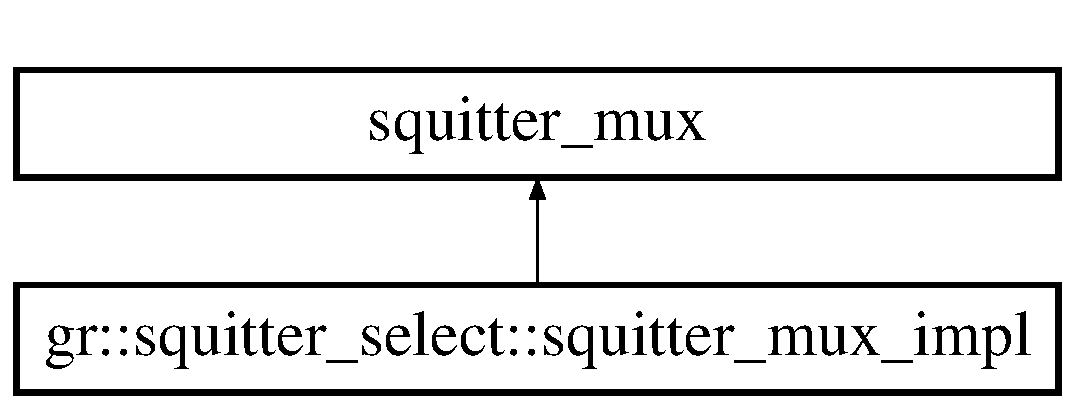
\includegraphics[height=2.000000cm]{classgr_1_1squitter__select_1_1squitter__mux__impl}
\end{center}
\end{figure}
\subsection*{Public Member Functions}
\begin{DoxyCompactItemize}
\item 
void {\bfseries set\+\_\+time} (pmt\+::pmt\+\_\+t msg)\hypertarget{classgr_1_1squitter__select_1_1squitter__mux__impl_afd37b0a2e8258decea7f334e4a2ef9fe}{}\label{classgr_1_1squitter__select_1_1squitter__mux__impl_afd37b0a2e8258decea7f334e4a2ef9fe}

\item 
pmt\+::pmt\+\_\+t {\bfseries msg} () const \hypertarget{classgr_1_1squitter__select_1_1squitter__mux__impl_aeabc800a78f1537d15d3a89231e88039}{}\label{classgr_1_1squitter__select_1_1squitter__mux__impl_aeabc800a78f1537d15d3a89231e88039}

\item 
{\bfseries squitter\+\_\+mux\+\_\+impl} (const std\+::string lengthname)\hypertarget{classgr_1_1squitter__select_1_1squitter__mux__impl_aaf4cd57c754c4ef7ee1688e441b0c839}{}\label{classgr_1_1squitter__select_1_1squitter__mux__impl_aaf4cd57c754c4ef7ee1688e441b0c839}

\item 
int {\bfseries work} (int noutput\+\_\+items, gr\+\_\+vector\+\_\+int \&ninput\+\_\+items, gr\+\_\+vector\+\_\+const\+\_\+void\+\_\+star \&input\+\_\+items, gr\+\_\+vector\+\_\+void\+\_\+star \&output\+\_\+items)\hypertarget{classgr_1_1squitter__select_1_1squitter__mux__impl_aa3f637f5f4ccc5eb32c9d8738f50a529}{}\label{classgr_1_1squitter__select_1_1squitter__mux__impl_aa3f637f5f4ccc5eb32c9d8738f50a529}

\end{DoxyCompactItemize}
\subsection*{Protected Member Functions}
\begin{DoxyCompactItemize}
\item 
int {\bfseries calculate\+\_\+output\+\_\+stream\+\_\+length} (const gr\+\_\+vector\+\_\+int \&ninput\+\_\+items)\hypertarget{classgr_1_1squitter__select_1_1squitter__mux__impl_a68044c9738e049bf45daf21148c203ec}{}\label{classgr_1_1squitter__select_1_1squitter__mux__impl_a68044c9738e049bf45daf21148c203ec}

\end{DoxyCompactItemize}


The documentation for this class was generated from the following files\+:\begin{DoxyCompactItemize}
\item 
squitter\+\_\+mux\+\_\+impl.\+h\item 
\hyperlink{squitter__mux__impl_8cc}{squitter\+\_\+mux\+\_\+impl.\+cc}\end{DoxyCompactItemize}

\chapter{File Documentation}
\hypertarget{squitter__mux__impl_8cc}{}\section{squitter\+\_\+mux\+\_\+impl.\+cc File Reference}
\label{squitter__mux__impl_8cc}\index{squitter\+\_\+mux\+\_\+impl.\+cc@{squitter\+\_\+mux\+\_\+impl.\+cc}}
{\ttfamily \#include $<$gnuradio/io\+\_\+signature.\+h$>$}\\*
{\ttfamily \#include \char`\"{}squitter\+\_\+mux\+\_\+impl.\+h\char`\"{}}\\*
\subsection*{Variables}
\begin{DoxyCompactItemize}
\item 
unsigned char {\bfseries apos\+\_\+odd} \mbox{[}P\+\_\+\+L\+EN\mbox{]}\hypertarget{squitter__mux__impl_8cc_ac979e6edc96ac90ec2a1c96ece0e6fa9}{}\label{squitter__mux__impl_8cc_ac979e6edc96ac90ec2a1c96ece0e6fa9}

\item 
unsigned char {\bfseries apos\+\_\+even} \mbox{[}P\+\_\+\+L\+EN\mbox{]}\hypertarget{squitter__mux__impl_8cc_ac2c8c0e53e0c134b9682b0773cae9cc6}{}\label{squitter__mux__impl_8cc_ac2c8c0e53e0c134b9682b0773cae9cc6}

\item 
unsigned char {\bfseries gpos\+\_\+odd} \mbox{[}P\+\_\+\+L\+EN\mbox{]}\hypertarget{squitter__mux__impl_8cc_a916fad84858fe416f403831bdb62b749}{}\label{squitter__mux__impl_8cc_a916fad84858fe416f403831bdb62b749}

\item 
unsigned char {\bfseries gpos\+\_\+even} \mbox{[}P\+\_\+\+L\+EN\mbox{]}\hypertarget{squitter__mux__impl_8cc_a6f1efb9c69d0d0687b31dc9be868e0ae}{}\label{squitter__mux__impl_8cc_a6f1efb9c69d0d0687b31dc9be868e0ae}

\item 
unsigned char {\bfseries avel} \mbox{[}P\+\_\+\+L\+EN\mbox{]}\hypertarget{squitter__mux__impl_8cc_aa1fd47b22b5a376f8e49fdb964a49428}{}\label{squitter__mux__impl_8cc_aa1fd47b22b5a376f8e49fdb964a49428}

\item 
unsigned char {\bfseries aid} \mbox{[}P\+\_\+\+L\+EN\mbox{]}\hypertarget{squitter__mux__impl_8cc_a9a71f129074402f0600d5c9be5ca3aa7}{}\label{squitter__mux__impl_8cc_a9a71f129074402f0600d5c9be5ca3aa7}

\end{DoxyCompactItemize}


\subsection{Detailed Description}
\begin{DoxyAuthor}{Author}
Ranisavljevic Daniel 
\end{DoxyAuthor}

%--- End generated contents ---

% Index
\backmatter
\newpage
\phantomsection
\clearemptydoublepage
\addcontentsline{toc}{chapter}{Index}
\printindex

\end{document}
